\documentclass[11pt, a4paper, USenglish]{article} % change ``USenglish'' to ``norsk'' if applicable.

\usepackage{kyblab} % Contains all included packages. See kyblab.sty.
\usepackage{float} % [H]
\renewcommand{\vec}[1]{\mathbf{#1}}
%matlab2tikz
\usepackage{pgfplots}
        \pgfplotsset{compat=newest}
        \pgfplotsset{plot coordinates/math parser=false}
\usepackage{tikz}
\usetikzlibrary{plotmarks}
  \usetikzlibrary{arrows.meta}
\usetikzlibrary{shapes.multipart}
\usepgfplotslibrary{patchplots}
\usepackage{grffile}
\newlength{\figureheight}
\newlength{\figurewidth}
%end matlab2tikz

\begin{document}
\subsection{Optimal Control of Pitch/Travel without Feedback}
\begin{figure}[H]
    \centering
    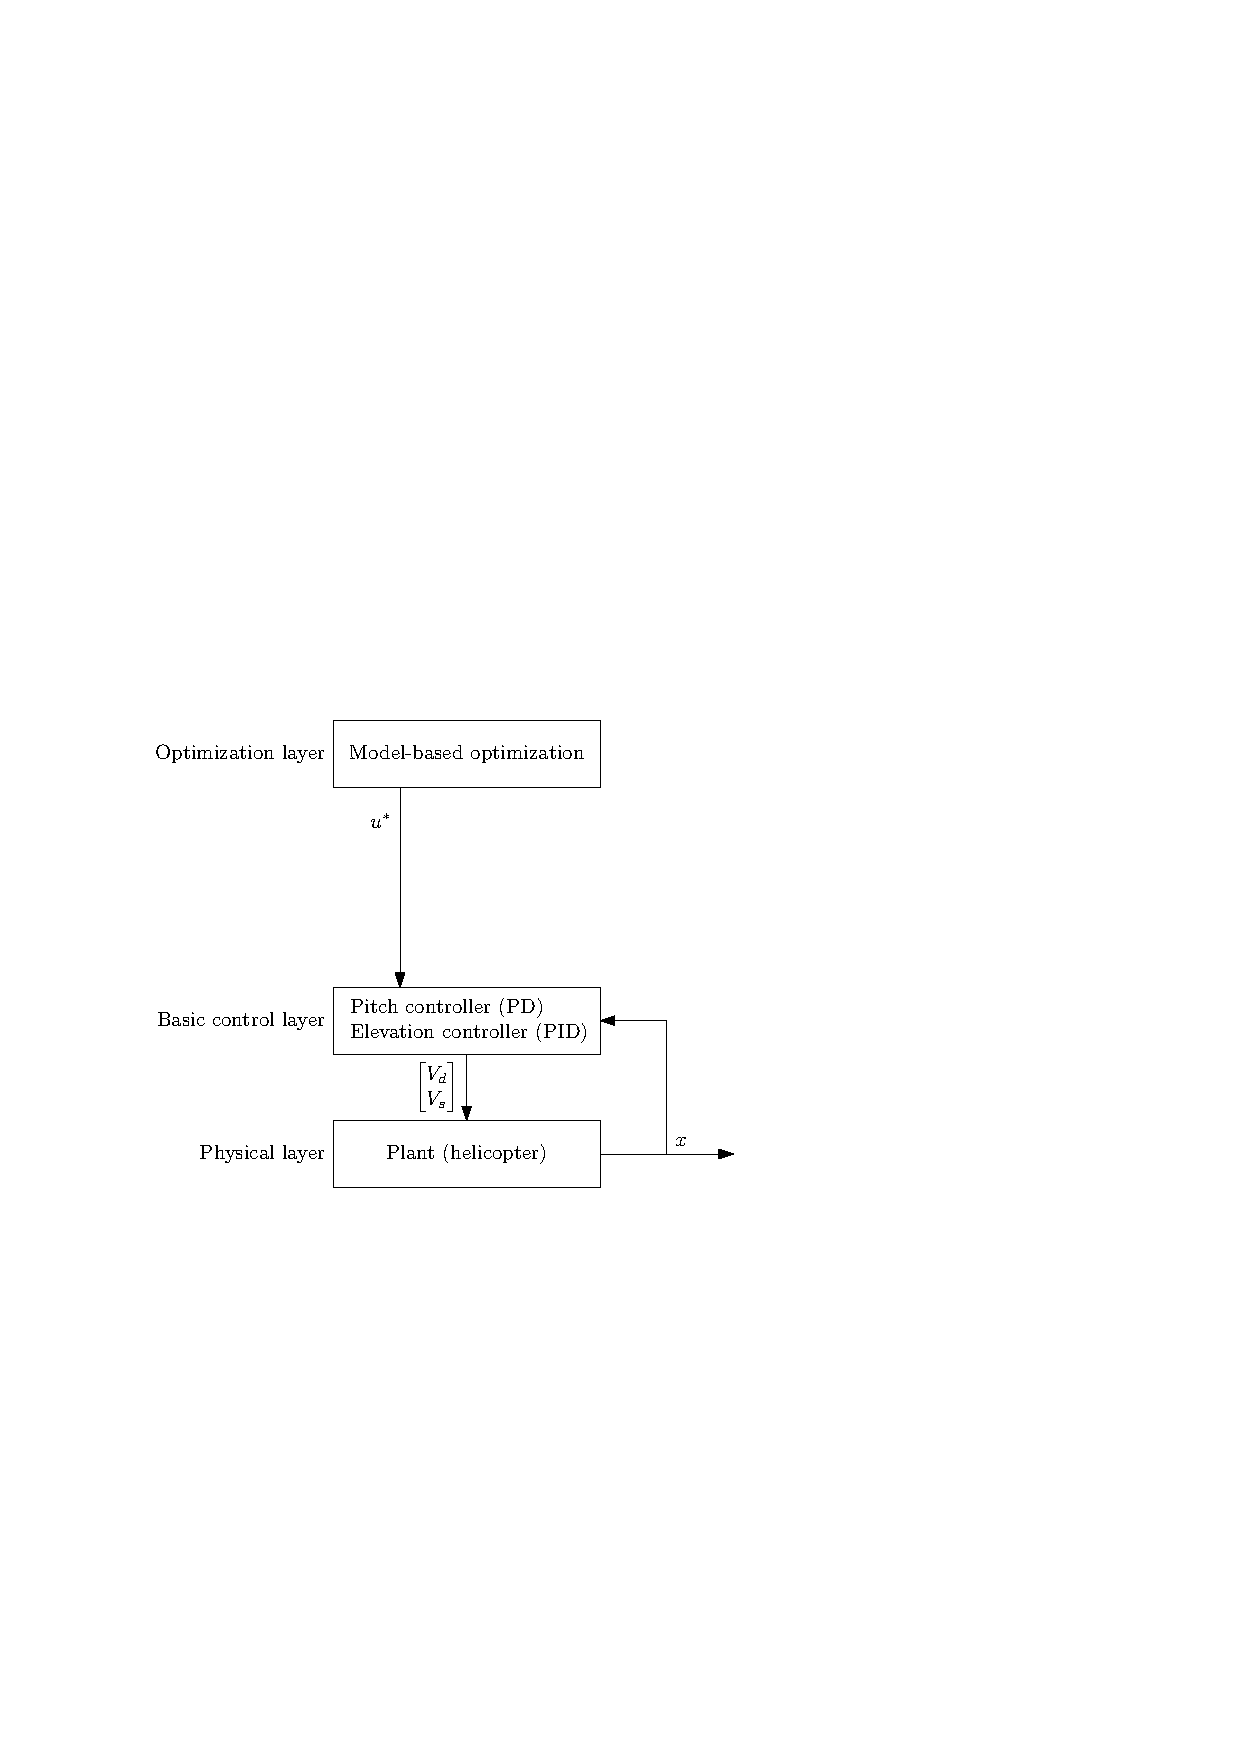
\includegraphics[width=1.00\textwidth]{figures/layers_openloop.pdf}
    \caption{A figure created with Ipe for TTK4135.}
\label{fig:layers_openloop}
\end{figure}

\begin{equation}
    \vec{\dot{x}} = A_c\vec{x} + B_c \vec{u} 
\end{equation}

\begin{equation*}
A_c =
    \begin{bmatrix}
        0 &  1 &  0 & 0 \\
        0 &  0 &  -K_2 & 0  \\
        0 &  0 &  0 & 1 \\
        0 &  0 & -K_1K_{pp} & -K_1K_{pd}                                 
    \end{bmatrix}
    , \quad B_c = 
    \begin{bmatrix} 0 \\ 0 \\ 0 \\ K_1K_{pp} \end{bmatrix}
\end{equation*}

\begin{align*}
    \vec{x_{k+1}} &= \vec{x_k} + h\vec{\dot{x}_k} \\
                  &= \vec{x_k} + h(A_c\vec{x_k} + B_c \vec{u_k}) \\  
                  &= (I + hA_C)\vec{x_k} + hB_c \vec{u_k} \\  
\end{align*}

\begin{figure}[H] 
        \centering
        \setlength{\figureheight}{6cm}
        \setlength{\figurewidth}{10cm}
        % This file was created by matlab2tikz.
%
%The latest updates can be retrieved from
%  http://www.mathworks.com/matlabcentral/fileexchange/22022-matlab2tikz-matlab2tikz
%where you can also make suggestions and rate matlab2tikz.
%
\definecolor{mycolor1}{rgb}{1.00000,0.00000,1.00000}%
%
\begin{tikzpicture}

\begin{axis}[%
width=0.951\figurewidth,
height=\figureheight,
at={(0\figurewidth,0\figureheight)},
scale only axis,
every outer x axis line/.append style={black},
every x tick label/.append style={font=\color{black}},
xmin=0,
xmax=35,
xlabel={Time [s]},
every outer y axis line/.append style={black},
every y tick label/.append style={font=\color{black}},
ymin=-1,
ymax=3.5,
ylabel={$\text{u, }\lambda\text{ [rad]}$},
axis background/.style={fill=white},
title={Weight q = 0.1},
axis x line*=bottom,
axis y line*=left,
legend style={legend cell align=left,align=left,draw=black}
]
\addplot[const plot,color=blue,solid] plot table[row sep=crcr] {%
0	0\\
0.25	0\\
0.5	0\\
0.75	0\\
1	0\\
1.25	0\\
1.5	0\\
1.75	0\\
2	0\\
2.25	0\\
2.5	0\\
2.75	0\\
3	0\\
3.25	0\\
3.5	0\\
3.75	0\\
4	0\\
4.25	0\\
4.5	0\\
4.75	0\\
5	0.523598775598074\\
5.25	0.523598775598034\\
5.5	0.523598775597983\\
5.75	0.523598775597915\\
6	0.523598775597823\\
6.25	0.523598775597692\\
6.5	0.523598775597497\\
6.75	0.523598775597182\\
7	0.523598775596606\\
7.25	0.523598775595267\\
7.5	0.523598775589254\\
7.75	0.388605461895739\\
8	0.10951698887527\\
8.25	-0.110038339461022\\
8.5	-0.276911237552916\\
8.75	-0.397906827316469\\
9	-0.479636751279011\\
9.25	-0.523591909441963\\
9.5	-0.523598775343426\\
9.75	-0.523598775363433\\
10	-0.523598722414531\\
10.25	-0.503434893916266\\
10.5	-0.464970440433064\\
10.75	-0.420773458613526\\
11	-0.373478625554464\\
11.25	-0.32522986550994\\
11.5	-0.277723446822207\\
11.75	-0.23225530276674\\
12	-0.189770188173245\\
12.25	-0.150910740882838\\
12.5	-0.116064946577637\\
12.75	-0.0854108906849835\\
13	-0.0589580160110363\\
13.25	-0.0365843889433275\\
13.5	-0.0180697126514252\\
13.75	-0.00312401628611978\\
14	0.0085879009858575\\
14.25	0.0174260785786064\\
14.5	0.0237587809673789\\
14.75	0.0279493320089856\\
15	0.0303460343335946\\
15.25	0.0312747968277704\\
15.5	0.0310340938210644\\
15.75	0.0298918916543043\\
16	0.0280841989107185\\
16.25	0.0258149231897645\\
16.5	0.0232567477403919\\
16.75	0.0205527737516956\\
17	0.0178187071682619\\
17.25	0.0151454014055185\\
17.5	0.0126015984112879\\
17.75	0.0102367395172331\\
18	0.00808374401737152\\
18.25	0.00616167714278127\\
18.5	0.00447824995691099\\
18.75	0.00303211167359721\\
19	0.00181491008787609\\
19.25	0.000813108362100164\\
19.5	9.55652768421745e-06\\
19.75	-0.000615176022881656\\
20	-0.00108169482085181\\
20.25	-0.00141088489524046\\
20.5	-0.00162320634848339\\
20.75	-0.00173816006303826\\
21	-0.00177390207933103\\
21.25	-0.00174698538733233\\
21.5	-0.00167220868418209\\
21.75	-0.00156255290812047\\
22	-0.0014291879259838\\
22.25	-0.00128153351051757\\
22.5	-0.00112736059780635\\
22.75	-0.000972920686000228\\
23	-0.000823093062976664\\
23.25	-0.000681541286448394\\
23.5	-0.000550871952314935\\
23.75	-0.000432790254030426\\
24	-0.000328248145159256\\
24.25	-0.000237582064620324\\
24.5	-0.000160638171127123\\
24.75	-9.68838666457343e-05\\
25	-4.55050786779726e-05\\
25.25	-5.48933099237643e-06\\
25.5	2.43049226562372e-05\\
25.75	4.50918802708431e-05\\
26	5.8113799538616e-05\\
26.25	6.46069335734721e-05\\
26.5	6.57765222737536e-05\\
26.75	6.27792011280751e-05\\
27	5.67109984837793e-05\\
27.25	4.85988379814542e-05\\
27.5	3.93931031714662e-05\\
27.75	2.99583230120062e-05\\
28	2.10584099342284e-05\\
28.25	1.33322661490434e-05\\
28.5	7.25543918037023e-06\\
28.75	3.08509956999618e-06\\
29	7.91904987941527e-07\\
29.25	-4.05937439716459e-17\\
29.5	-1.53321449279011e-17\\
29.75	0\\
30	0\\
30.25	0\\
30.5	0\\
30.75	0\\
31	0\\
31.25	0\\
31.5	0\\
31.75	0\\
32	0\\
32.25	0\\
32.5	0\\
32.75	0\\
33	0\\
33.25	0\\
33.5	0\\
33.75	0\\
34	0\\
34.25	0\\
34.5	0\\
34.75	0\\
35	0\\
};
\addlegendentry{$\text{p}_\text{c}$};

\addplot [color=mycolor1,solid]
  table[row sep=crcr]{%
0	3.14159265358979\\
0.25	3.14159265358979\\
0.5	3.14159265358979\\
0.75	3.14159265358979\\
1	3.14159265358979\\
1.25	3.14159265358979\\
1.5	3.14159265358979\\
1.75	3.14159265358979\\
2	3.14159265358979\\
2.25	3.14159265358979\\
2.5	3.14159265358979\\
2.75	3.14159265358979\\
3	3.14159265358979\\
3.25	3.14159265358979\\
3.5	3.14159265358979\\
3.75	3.14159265358979\\
4	3.14159265358979\\
4.25	3.14159265358979\\
4.5	3.14159265358979\\
4.75	3.14159265358979\\
5	3.14159265358979\\
5.25	3.14159265358979\\
5.5	3.14159265358979\\
5.75	3.14159265358979\\
6	3.13784214136253\\
6.25	3.126215553458\\
6.5	3.10330930002998\\
6.75	3.06662741519122\\
7	3.01445392239423\\
7.25	2.94565627711768\\
7.5	2.85950776329371\\
7.75	2.75555158796541\\
8	2.63350511049065\\
8.25	2.49319560603263\\
8.5	2.33451857606511\\
8.75	2.15837827192605\\
9	1.96780007787047\\
9.25	1.76741104454662\\
9.5	1.56258105127613\\
9.75	1.35868396793868\\
10	1.16059209032489\\
10.25	0.972354196797713\\
10.5	0.796950123259841\\
10.75	0.636432933749591\\
11	0.492159597969274\\
11.25	0.36485729820996\\
11.5	0.25463993267206\\
11.75	0.161096235930179\\
12	0.0834005912521931\\
12.25	0.0204236245333906\\
12.5	-0.0291675128159417\\
12.75	-0.0668230046530649\\
13	-0.0940391853047939\\
13.25	-0.112301690219796\\
13.5	-0.123041675965191\\
13.75	-0.127603583533352\\
14	-0.127222853792057\\
14.25	-0.123012039483811\\
14.5	-0.115953847476759\\
14.75	-0.106899763407816\\
15	-0.0965730445362397\\
15.25	-0.0855750068726116\\
15.5	-0.0743936735427865\\
15.75	-0.0634139886026101\\
16	-0.0529289309785858\\
16.25	-0.0431509845929514\\
16.5	-0.034223531491126\\
16.75	-0.0262318339987593\\
17	-0.0192133591912855\\
17.25	-0.0131672742880113\\
17.5	-0.00806300535517535\\
17.75	-0.00384780454936746\\
18	-0.0004533138735938\\
18.25	0.00219885300364836\\
18.5	0.0041924638884134\\
18.75	0.00561289086980216\\
19	0.00654412528516249\\
19.25	0.00706650021892946\\
19.5	0.00725503299040899\\
19.75	0.00717830051005529\\
20	0.00689776339525422\\
20.25	0.00646745966611192\\
20.5	0.00593399511017771\\
20.75	0.00533676452114737\\
21	0.00470834557251294\\
21.25	0.00407501475230339\\
21.5	0.00345734229922592\\
21.75	0.00287083024602222\\
22	0.00232656434980062\\
22.25	0.00183185677553755\\
22.5	0.00139086184134206\\
22.75	0.00100515190830851\\
23	0.000674244605617742\\
23.25	0.0003960760448359\\
23.5	0.000167417532882236\\
23.75	-1.57644118584706e-05\\
24	-0.000158003147386422\\
24.25	-0.000264079167713\\
24.5	-0.000338815653456829\\
24.75	-0.000386917817245833\\
25	-0.000412851210807727\\
25.25	-0.000420754050890027\\
25.5	-0.000414378691834756\\
25.75	-0.000397057581793275\\
26	-0.000371689350269946\\
26.25	-0.000340741054982522\\
26.5	-0.000306263038766121\\
26.75	-0.000269913289732788\\
27	-0.00023298864146416\\
27.25	-0.00019646057949526\\
27.5	-0.000161013823462394\\
27.75	-0.000127086220927492\\
28	-9.49088102821858e-05\\
28.25	-6.45451778638679e-05\\
28.5	-3.5929439305405e-05\\
28.75	-8.90230607054183e-06\\
29	1.67552588483429e-05\\
29.25	4.12913533646134e-05\\
29.5	6.49561545002824e-05\\
29.75	8.79796792978908e-05\\
30	0.00011055569399486\\
30.25	0\\
30.5	0\\
30.75	0\\
31	0\\
31.25	0\\
31.5	0\\
31.75	0\\
32	0\\
32.25	0\\
32.5	0\\
32.75	0\\
33	0\\
33.25	0\\
33.5	0\\
33.75	0\\
34	0\\
34.25	0\\
34.5	0\\
34.75	0\\
35	0\\
};
\addlegendentry{$\lambda$};

\addplot [color=mycolor1,solid,forget plot]
  table[row sep=crcr]{%
0	3.14159265358979\\
0.25	3.14159265358979\\
0.5	3.14159265358979\\
0.75	3.14159265358979\\
1	3.14159265358979\\
1.25	3.14159265358979\\
1.5	3.14159265358979\\
1.75	3.14159265358979\\
2	3.14159265358979\\
2.25	3.14159265358979\\
2.5	3.14159265358979\\
2.75	3.14159265358979\\
3	3.14159265358979\\
3.25	3.14159265358979\\
3.5	3.14159265358979\\
3.75	3.14159265358979\\
4	3.14159265358979\\
4.25	3.14159265358979\\
4.5	3.14159265358979\\
4.75	3.14159265358979\\
5	3.14159265358979\\
5.25	3.14159265358979\\
5.5	3.14159265358979\\
5.75	3.14159265358979\\
6	3.13784214136253\\
6.25	3.126215553458\\
6.5	3.10330930002998\\
6.75	3.06662741519122\\
7	3.01445392239423\\
7.25	2.94565627711768\\
7.5	2.85950776329371\\
7.75	2.75555158796541\\
8	2.63350511049065\\
8.25	2.49319560603263\\
8.5	2.33451857606511\\
8.75	2.15837827192605\\
9	1.96780007787047\\
9.25	1.76741104454662\\
9.5	1.56258105127613\\
9.75	1.35868396793868\\
10	1.16059209032489\\
10.25	0.972354196797713\\
10.5	0.796950123259841\\
10.75	0.636432933749591\\
11	0.492159597969274\\
11.25	0.36485729820996\\
11.5	0.25463993267206\\
11.75	0.161096235930179\\
12	0.0834005912521931\\
12.25	0.0204236245333906\\
12.5	-0.0291675128159417\\
12.75	-0.0668230046530649\\
13	-0.0940391853047939\\
13.25	-0.112301690219796\\
13.5	-0.123041675965191\\
13.75	-0.127603583533352\\
14	-0.127222853792057\\
14.25	-0.123012039483811\\
14.5	-0.115953847476759\\
14.75	-0.106899763407816\\
15	-0.0965730445362397\\
15.25	-0.0855750068726116\\
15.5	-0.0743936735427865\\
15.75	-0.0634139886026101\\
16	-0.0529289309785858\\
16.25	-0.0431509845929514\\
16.5	-0.034223531491126\\
16.75	-0.0262318339987593\\
17	-0.0192133591912855\\
17.25	-0.0131672742880113\\
17.5	-0.00806300535517535\\
17.75	-0.00384780454936746\\
18	-0.0004533138735938\\
18.25	0.00219885300364836\\
18.5	0.0041924638884134\\
18.75	0.00561289086980216\\
19	0.00654412528516249\\
19.25	0.00706650021892946\\
19.5	0.00725503299040899\\
19.75	0.00717830051005529\\
20	0.00689776339525422\\
20.25	0.00646745966611192\\
20.5	0.00593399511017771\\
20.75	0.00533676452114737\\
21	0.00470834557251294\\
21.25	0.00407501475230339\\
21.5	0.00345734229922592\\
21.75	0.00287083024602222\\
22	0.00232656434980062\\
22.25	0.00183185677553755\\
22.5	0.00139086184134206\\
22.75	0.00100515190830851\\
23	0.000674244605617742\\
23.25	0.0003960760448359\\
23.5	0.000167417532882236\\
23.75	-1.57644118584706e-05\\
24	-0.000158003147386422\\
24.25	-0.000264079167713\\
24.5	-0.000338815653456829\\
24.75	-0.000386917817245833\\
25	-0.000412851210807727\\
25.25	-0.000420754050890027\\
25.5	-0.000414378691834756\\
25.75	-0.000397057581793275\\
26	-0.000371689350269946\\
26.25	-0.000340741054982522\\
26.5	-0.000306263038766121\\
26.75	-0.000269913289732788\\
27	-0.00023298864146416\\
27.25	-0.00019646057949526\\
27.5	-0.000161013823462394\\
27.75	-0.000127086220927492\\
28	-9.49088102821858e-05\\
28.25	-6.45451778638679e-05\\
28.5	-3.5929439305405e-05\\
28.75	-8.90230607054183e-06\\
29	1.67552588483429e-05\\
29.25	4.12913533646134e-05\\
29.5	6.49561545002824e-05\\
29.75	8.79796792978908e-05\\
30	0.00011055569399486\\
30.25	0\\
30.5	0\\
30.75	0\\
31	0\\
31.25	0\\
31.5	0\\
31.75	0\\
32	0\\
32.25	0\\
32.5	0\\
32.75	0\\
33	0\\
33.25	0\\
33.5	0\\
33.75	0\\
34	0\\
34.25	0\\
34.5	0\\
34.75	0\\
35	0\\
};
\end{axis}
\end{tikzpicture}%
        \caption{test} 
\label{fig:figure1} 
\end{figure}


\end{document}
